%-----------------------------------------------
% Template para criação de resumos de projectos/dissertação
% jlopes AT fe.up.pt,   Fri Jul  3 11:08:59 2009
%-----------------------------------------------

\documentclass[9pt,a4paper]{extarticle}

%% English version: comment first, uncomment second
%\usepackage[portuguese]{babel}  % Portuguese
\usepackage[english]{babel}     % English
\usepackage{graphicx}           % images .png or .pdf w/ pdflatex OR .eps w/ latex
\usepackage{times}              % use Times type-1 fonts
\usepackage[utf8]{inputenc}     % 8 bits using UTF-8
\usepackage{url}                % URLs
\usepackage{multicol}           % twocolumn, etc
\usepackage{float}              % improve figures & tables floating
\usepackage[tableposition=top]{caption} % captions
%% English version: comment first (maybe)
\usepackage{indentfirst}        % portuguese standard for paragraphs
\usepackage{subfig}
%\usepackage{parskip}

%% page layout
\usepackage[a4paper,margin=30mm,noheadfoot]{geometry}

%% space between columns
\columnsep 12mm

%% headers & footers
\pagestyle{empty}

%% figure & table caption
\captionsetup{figurename=Fig.,tablename=Tab.,labelsep=endash,font=bf,skip=.5\baselineskip}

%% heading
\makeatletter
\renewcommand*{\@seccntformat}[1]{%
  \csname the#1\endcsname.\quad
}
\makeatother

%% avoid widows and orphans
\clubpenalty=300
\widowpenalty=300

\begin{document}

\title{\vspace*{-8mm}\textbf{\textsc{End-User Programming in Mobile Devices
through Re-usable Visual Components Composition}}
\author{\emph{Tiago Manuel da Silva Almeida}\\[2mm]
\small{Dissertation supervised by \emph{Prof.\ Hugo Sereno Ferreira}}\\
\small{and co-supervised by Tiago Boldt Sousa}}}
\date{}
\maketitle
%no page number 
\thispagestyle{empty}

\vspace*{-4mm}\noindent\rule{\textwidth}{0.4pt}\vspace*{4mm}

\begin{multicols}{2}

\section{Motivation}\label{sec:motiva}

An era where smartphones surpassed the PCs sales has begun \cite{more_smartphones}. In this era, the end-users (the ones that ultimately use the smartphone) 
are demanding quantity and complexity from their applications and devices. 
This makes it impractical for a software developer to ``foresee'' every possible combination and explore every valid alternative.

A possible solution is to empower end-users with \emph{end-user programming} (EUP) tools. 
The main difference between an end-user programmer and a professional programmer is the target user \cite{SotaEUE2011}. 
A professional programmer programs for an external user, while an end-user programmer programs for himself.
We can conceive a EUP tool that allows the end-users to explore their necessities in a collaborative framework, where novices and experts can co-exist and share. Expert programmers can
create the components, and end-users can connect them using a \emph{visual programming language} (VPL).
We believe that such a tool could not only reduce the number of ``small'', specific-tailored applications, but also foster discovery and experimentation.

\section{Objectives}\label{sec:goals}

We studied the following topics: 

\begin{itemize}
	\item{\textbf{Smartphone's limitations in the implementation of a EUP solution} \\
    VPLs can be hard to use in a small screen. How can we use visual elements without overflooding the screen? A solution with zoom is enough?
	Can we use VPLs in a small screen and work with solutions with a medium-large amount of components?}
	
	\item{\textbf{Defining an abstraction level for a collaborative framework} \\
	Low abstraction levels may be good for end-users but they can limit the blocks that can be produced by expert programmers.
	Can we achieve a good abstraction level for both end-users and expert programmers?}
  
	\item{\textbf{Impact of the reuse in EUP} \\
    How can we approach reuse and incentive end-users to use it?
    Do we need a market just for components reusing? 
	Sharing is the only reuse option or there are other options?}
	
	\item{\textbf{Study of a collaborative environment between EUP and expert programmers} \\
    Does a collaborative environment help end-users? Should end-users have a means to ask for components? 
    How can expert programmers benefit from this approach? 
    Do expert programmers also like to connect components instead of programming them?}
\end{itemize}


\section{From Android to Scala: Steps into a EUP solution}\label{sec:work}

We started to look into EUP problems \cite{Barriers2004} and then, we explored another area: \emph{End-User Software Engineering} (EUSE).
Additionally, we found out that VPLs can be used to solve some of those problems, so we also studied this kind of languages.

A prototype for Android using concepts from VPLs was developed and improved with end-users feedback. 

Next we decided to experiment a new language to solve some problems pointed out by end-users: Scala \cite{ProgrammingScala}.

\subsection{A typed block-based prototype}

\begin{figure}[H]
\centerline{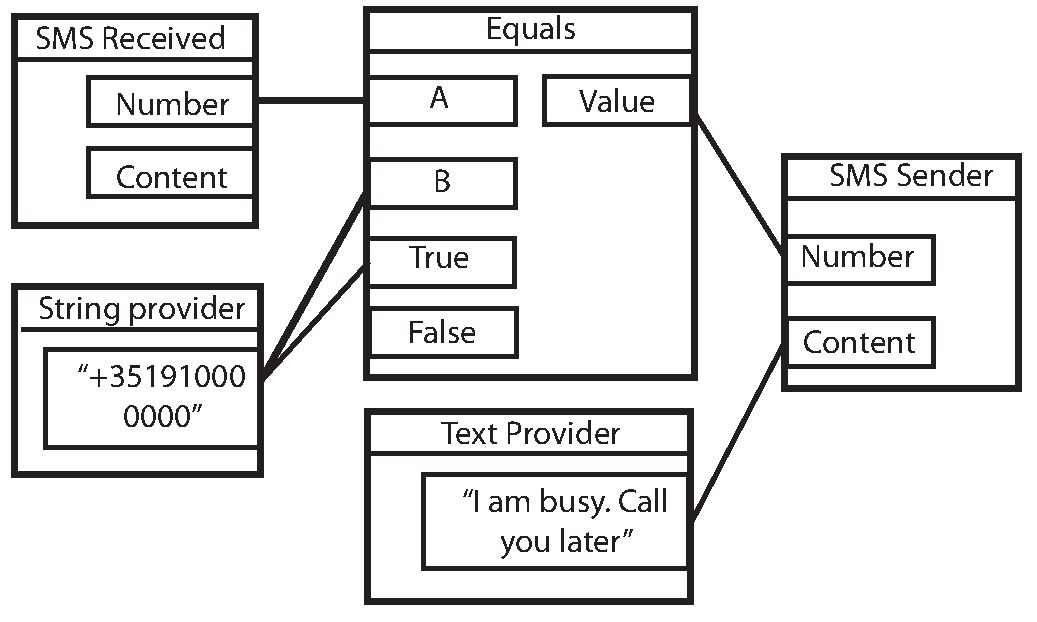
\includegraphics[scale=.43]{block_example.pdf}}
\label{fig:block}
\caption{A task composed by a set of blocks.} 
\end{figure}

A block with inputs and outputs is a common representation in software engineering. 
Black box testing, for instance, uses this metaphor. 
This metaphor was also thought for EUP, and it was described by Zin in a recent paper \cite{Zin2011}. 
The main idea is: We have a block, with a set of inputs and it returns data into outputs that can be connected with inputs.
Both outputs and inputs are called connectors and each connector has a type. A set of connected blocks is a block. 

A block  can be shown to the end-user using a box with inputs on the left and outputs on the right. 
Figure \ref{fig:block} shows that a block can connect its outputs with inputs from other block. This figure shows a task that automatically replies a message with the content ``I am busy. Call you later'' when a message is received from the number ``+351910000000''. The equal blocks has two set of inputs: \texttt{A} and  \texttt{B}, that are the values to be compared; \texttt{True} and  \texttt{Flase},
that are the values that will be used in case the expression \texttt{A == B} is true or false. The \texttt{Value} output will hold the value from  \texttt{True} or  \texttt{False} is send in the  .
Blocks can be developed by expert programmers and end-users can connect and share them. 
A set of connected blocks creates a task, and a task is, itself, a block that can be connected with other blocks.

\subsection{Experiments with a rewrite rule system}

Some improvements were made in the prototype that were based on end-users' feedback, but they weren't enough.
We needed a way to do automatic simplifications in a set of blocks, and other way to convert connectors' types without recurring
to extra blocks. We tried to use Scala to solve this problems.

Scala has two main features that called our attention: pattern matching and implicit conversions. Pattern matching allow us to search for patterns in a set of connected blocks in an easy way, and implicit conversions let us define some conversions without the need to do casts. In Java, if we want to convert from a \texttt{String} to an \texttt{Integer} we can do: Integer.parseInt(string). In Scala we can define an implicit,
and every time a \texttt{String} is used and a Integer was expected, the implicit will be called.

With this two features we created a rewrite rule system. This system was made so it could automatically simplify situations like:
If a set of block has two constants being summed then create a constant to replace it. In fact, there is no actual replacement,
only a visual abstraction. 

\section{Conclusions}\label{sec:conclui}

We couldn't use our rewrite rule system because the integration with Scala in Android didn't work as we expected.
However, our prototype is fully functional and it can be used to do more tests with end-users.
We developed a solution for visual overflow that could happen using a VPL in a smartphone. 

We collected some feedback from end-users that allowed us to understand what they priorities are.
We noticed that end-users prefer tasks that have a small amount of blocks. They are not worried with the potentialities
the system has. Also, we had to do a tutorial to explain some of the concepts involved and our task creation process. Some end-users couldn't understand all concepts at the first usage, but a small oral explanation usually was enough. 

%%English version: comment first, uncomment second
%\bibliographystyle{unsrt-pt}  % numeric, unsorted refs
\bibliographystyle{unsrt}  % numeric, unsorted refs
\bibliography{refs}

\end{multicols}

\end{document}
